\documentclass[12pt]{article}

\usepackage{sbc-template}
\usepackage{graphicx,url}
\usepackage[utf8]{inputenc}
\usepackage[brazil]{babel}
\usepackage[latin1]{inputenc}
\title{Algoritmos de Busca no Pac-Man \\ Introdução à Inteligência Artificial}

\author{Vinicius Julião Ramos - 2018054630}


\address{Departamento de Ciência da Computação \\Universidade Federal de Minas Gerais
  (UFMG)
  \email{viniciusjuliao@dcc.ufmg.br}
}
\maketitle
\begin{document} 

\section{Introdução}

O presente trabalho constituído pelo desenvolvimento e análise da aplicação
de algoritmos de busca sobre o jogo Pac-Man.
Essa atividade tem como fim a introdução de algoritmos utilizados por
inteligências artificiais em problemas reais, como um \textit{video game}.
Além disso, tal aplicação só é possível graças à modelagem do problema, em que
o estado do jogo se dá pelas posições disponíveis no tabuleiro (mapa),
sendo que os estados considerados como estados objetivos, são aqueles que
contêm a "comida" do personagem.

No jogo, o personagem pode mudar de posição apenas para aquelas posições
ajacentes à posição atual.
Tal adjacência se dá pelas posições acima, abaixo, à esquerda e à direita.
Logo, cada estado tem no máximo quatro outros estados descendentes.
É importante destacar que o mapa não é infinito, ou seja, há barreiras que
impedem o personagem de realizar um movimento, logo é possível que
determinados estados tenham menos de quatro estados descendentes.
Dessa forma, é possível caminhar de forma sistêmica em todo este grafo a fim
de alcançar os estados objetivos, e vencer o jogo.

Apesar da simplicidade do solucionador de um jogo 2D, a busca em grafos é
utilizada em diversas aplicações muito complexas, mas que em linhas gerais tem
uma implementação relativamente simples.
Um outro fator de importância dos algoritmos de busca, é que são adaptáveis a
diferentes tipos de problemas, em que alguns são mais genéricos, outros mais
possuem maio conversão de especificidade.
Um bom exemplo são os algoritmos \textbf{BFS} e \textbf{A*}, em que o primeiro
pode ser aplicado de maneira genérica em muitos tipos de busca em grafos.
Já o segundo algoritmo, demanda a criação de uma função heurística, o que
desperta a necessidade do entendimento do comportamento das instancias
que o algoritmo resolve, a fim de que essa função heurística seja capaz
de optimiza a busca.


\section{First Page} \label{sec:firstpage}

The first page must display the paper title, the name and address of the
authors, the abstract in English and ``resumo'' in Portuguese (``resumos'' are
required only for papers written in Portuguese). The title must be centered
over the whole page, in 16 point boldface font and with 12 points of space
before itself. Author names must be centered in 12 point font, bold, all of
them disposed in the same line, separated by commas and with 12 points of
space after the title. Addresses must be centered in 12 point font, also with
12 points of space after the authors' names. E-mail addresses should be
written using font Courier New, 10 point nominal size, with 6 points of space
before and 6 points of space after.

The abstract and ``resumo'' (if is the case) must be in 12 point Times font,
indented 0.8cm on both sides. The word \textbf{Abstract} and \textbf{Resumo},
should be written in boldface and must precede the text.

\section{CD-ROMs and Printed Proceedings}

In some conferences, the papers are published on CD-ROM while only the
abstract is published in the printed Proceedings. In this case, authors are
invited to prepare two final versions of the paper. One, complete, to be
published on the CD and the other, containing only the first page, with
abstract and ``resumo'' (for papers in Portuguese).

\section{Sections and Paragraphs}

Section titles must be in boldface, 13pt, flush left. There should be an extra
12 pt of space before each title. Section numbering is optional. The first
paragraph of each section should not be indented, while the first lines of
subsequent paragraphs should be indented by 1.27 cm.

\subsection{Subsections}

The subsection titles must be in boldface, 12pt, flush left.

\section{Figures and Captions}\label{sec:figs}


Figure and table captions should be centered if less than one line
(Figure~\ref{fig:exampleFig1}), otherwise justified and indented by 0.8cm on
both margins, as shown in Figure~\ref{fig:exampleFig2}. The caption font must
be Helvetica, 10 point, boldface, with 6 points of space before and after each
caption.

\begin{figure}[ht]
\centering
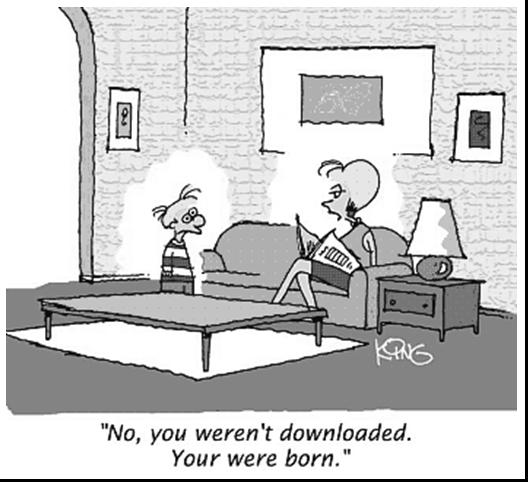
\includegraphics[width=.5\textwidth]{fig1.jpg}
\caption{A typical figure}
\label{fig:exampleFig1}
\end{figure}

\begin{figure}[ht]
\centering
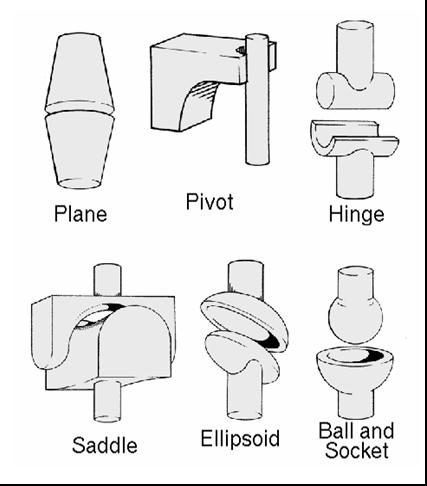
\includegraphics[width=.3\textwidth]{fig2.jpg}
\caption{This figure is an example of a figure caption taking more than one
  line and justified considering margins mentioned in Section~\ref{sec:figs}.}
\label{fig:exampleFig2}
\end{figure}

In tables, try to avoid the use of colored or shaded backgrounds, and avoid
thick, doubled, or unnecessary framing lines. When reporting empirical data,
do not use more decimal digits than warranted by their precision and
reproducibility. Table caption must be placed before the table (see Table 1)
and the font used must also be Helvetica, 10 point, boldface, with 6 points of
space before and after each caption.

\begin{table}[ht]
\centering
\caption{Variables to be considered on the evaluation of interaction
  techniques}
\label{tab:exTable1}
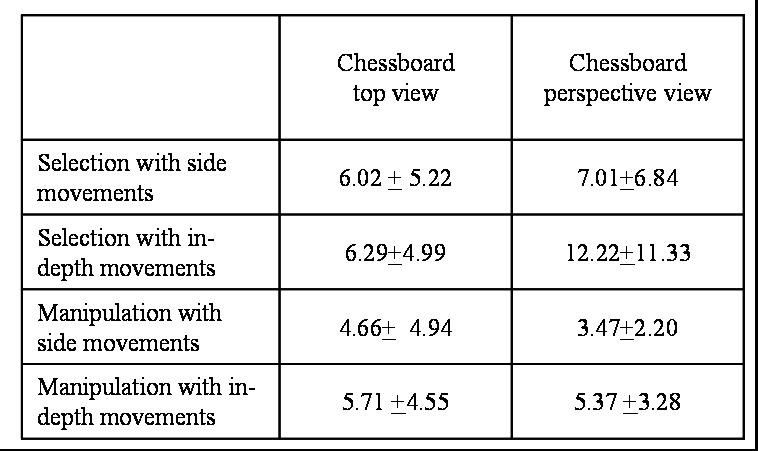
\includegraphics[width=.7\textwidth]{table.jpg}
\end{table}

\section{Images}

All images and illustrations should be in black-and-white, or gray tones,
excepting for the papers that will be electronically available (on CD-ROMs,
internet, etc.). The image resolution on paper should be about 600 dpi for
black-and-white images, and 150-300 dpi for grayscale images.  Do not include
images with excessive resolution, as they may take hours to print, without any
visible difference in the result. 

\section{References}

Bibliographic references must be unambiguous and uniform.  We recommend giving
the author names references in brackets, e.g. \cite{knuth:84},
\cite{boulic:91}, and \cite{smith:99}.

The references must be listed using 12 point font size, with 6 points of space
before each reference. The first line of each reference should not be
indented, while the subsequent should be indented by 0.5 cm.

\bibliographystyle{sbc}
\bibliography{sbc-template}

\end{document}
